\documentclass[a4paper,12pt]{article}

% Paquetes básicos
\usepackage[utf8]{inputenc}
\usepackage[T1]{fontenc}
\usepackage[spanish]{babel}
\usepackage{graphicx}
\usepackage{xcolor}
\usepackage{lipsum}
\usepackage{geometry}
\geometry{top=3cm, bottom=3cm, left=2.5cm, right=2.5cm}



% Paquetes para figuras
\usepackage{tikz}
\usetikzlibrary{positioning, arrows}
\usetikzlibrary{positioning, shapes.geometric, decorations.pathreplacing, arrows.meta}

% Define styles for the diagram
\tikzstyle{class} = [rectangle, draw, fill=blue!10, rounded corners, minimum height=2em, minimum width=4cm, text centered]
\tikzstyle{arrow} = [thick, ->, >=stealth]

% Paquetes para diseño
\usepackage{titlesec}
\usepackage{fancyhdr}
\usepackage{amsmath}
\usepackage{amssymb}
\usepackage{hyperref}

% Paquetes para el entorno lstlisting
\usepackage{listings}
\usepackage{inconsolata}

%encabezado y pie de página nivel profesional
\usepackage{fancyhdr}
\pagestyle{fancy}
\fancyhf{}
\fancyhead[L]{\leftmark}
\fancyhead[R]{\rightmark}
\fancyfoot[L]{\textbf{Ismael Sallami Moreno - GIIADE}}
\fancyfoot[C]{\thepage}
\fancyfoot[R]{\textbf{(UGR)} \today}
\renewcommand{\headrulewidth}{0.4pt}
\renewcommand{\footrulewidth}{0.4pt}
\setlength{\headheight}{15pt}
\setlength{\headsep}{10pt}
\setlength{\footskip}{20pt}
\usepackage{truncate}
\fancyhead[L]{\truncate{0.5\headwidth}{\leftmark}}
\fancyhead[R]{\truncate{0.5\headwidth}{\rightmark}}
\usepackage{mathpazo}
\usepackage{tcolorbox}


% Paquete para fondo
\usepackage{background}
\usepackage{float}

% Configuración de lstlisting
\lstset{
    inputencoding=utf8,          % Permite UTF-8
    extendedchars=true,          % Reconoce caracteres extendidos
    literate=                    % Configuración manual para tildes y símbolos
        {á}{{\'a}}1
        {é}{{\'e}}1
        {í}{{\'i}}1
        {ó}{{\'o}}1
        {ú}{{\'u}}1
        {ñ}{{\~n}}1
        {Á}{{\'A}}1
        {É}{{\'E}}1
        {Í}{{\'I}}1
        {Ó}{{\'O}}1
        {Ú}{{\'U}}1
        {Ñ}{{\~N}}1
        {¿}{{\textquestiondown}}1
        {¡}{{\textexclamdown}}1,
    basicstyle=\ttfamily,        % Fuente monoespaciada
    breaklines=true,             % Habilita salto de línea automático
    frame=single,                % Marco alrededor del código
    backgroundcolor=\color{gray!10}, % Fondo gris claro
    keywordstyle=\color{blue},   % Color para palabras clave
    commentstyle=\color{green},  % Color para comentarios
    stringstyle=\color{red}      % Color para strings
}
\lstdefinestyle{customcpp}{
    language=C++,                % Lenguaje de programación
    showspaces=false,            % No mostrar espacios
    showtabs=false,              % No mostrar tabulaciones
    tabsize=4,                   % Tamaño de tabulación
    showstringspaces=false,      % No mostrar espacios en strings
    numbers=left,                % Números de línea a la izquierda
    numberstyle=\tiny\color{gray}, % Estilo de los números de línea
    numbersep=5pt,               % Separación de los números de línea
    stepnumber=1,                % Mostrar número en cada línea
    basicstyle=\ttfamily\footnotesize, % Estilo básico del código
    keywordstyle=\bfseries\color{blue}, % Estilo de las palabras clave
    commentstyle=\itshape\color{green!50!black}, % Estilo de los comentarios
    stringstyle=\color{red},     % Estilo de los strings
    identifierstyle=\color{black}, % Estilo de los identificadores
    % procnamekeys={def,class},    % Palabras clave para nombres de funciones
    morekeywords={constexpr,nullptr,size_t}, % Más palabras clave
    emph={int,char,double,float,unsigned}, % Palabras a enfatizar
    emphstyle=\color{magenta},   % Estilo de las palabras enfatizadas
    backgroundcolor=\color{gray!10}, % Color de fondo
    frame=shadowbox,             % Marco con sombra
    rulesepcolor=\color{gray},   % Color de la línea de separación
    breakatwhitespace=false,     % No cortar en espacios en blanco
    breaklines=true,             % Cortar líneas largas
    captionpos=b,                % Posición del título (abajo)
    escapeinside={(*@}{@*)},     % Delimitadores para escapar a LaTeX
    morecomment=[l][\color{magenta}]{\#}, % Comentarios de una línea
    morecomment=[s][\color{orange}]{/*}{*/}, % Comentarios multilínea
    morestring=[b]",             % Strings entre comillas dobles
    morestring=[b]'              % Strings entre comillas simples
}
\lstdefinestyle{customjava}{
    language=Java,               % Lenguaje de programación
    showspaces=false,            % No mostrar espacios
    showtabs=false,              % No mostrar tabulaciones
    tabsize=4,                   % Tamaño de tabulación
    showstringspaces=false,      % No mostrar espacios en strings
    numbers=left,                % Números de línea a la izquierda
    numberstyle=\tiny\color{gray}, % Estilo de los números de línea
    numbersep=5pt,               % Separación de los números de línea
    stepnumber=1,                % Mostrar número en cada línea
    basicstyle=\ttfamily\footnotesize, % Estilo básico del código
    keywordstyle=\bfseries\color{purple}, % Estilo de las palabras clave
    commentstyle=\itshape\color{green!50!black}, % Estilo de los comentarios
    stringstyle=\color{orange},  % Estilo de los strings
    identifierstyle=\color{black}, % Estilo de los identificadores
    morekeywords={abstract, assert, boolean, break, byte, case, catch, char, class, const, continue, default, do, double, else, enum, extends, final, finally, float, for, goto, if, implements, import, instanceof, int, interface, long, native, new, null, package, private, protected, public, return, short, static, strictfp, super, switch, synchronized, this, throw, throws, transient, try, void, volatile, while}, % Más palabras clave
    emph={int,char,double,float,unsigned}, % Palabras a enfatizar
    emphstyle=\color{magenta},   % Estilo de las palabras enfatizadas
    backgroundcolor=\color{gray!10}, % Color de fondo
    frame=shadowbox,             % Marco con sombra
    rulesepcolor=\color{gray},   % Color de la línea de separación
    breakatwhitespace=false,     % No cortar en espacios en blanco
    breaklines=true,             % Cortar líneas largas
    captionpos=b,                % Posición del título (abajo)
    escapeinside={(*@}{@*)},     % Delimitadores para escapar a LaTeX
    morecomment=[l][\color{magenta}]{\#}, % Comentarios de una línea
    morecomment=[s][\color{orange}]{/*}{*/}, % Comentarios multilínea
    morestring=[b]",             % Strings entre comillas dobles
    morestring=[b]'              % Strings entre comillas simples
}

\lstdefinestyle{customrb}{
    language=Ruby,               % Lenguaje de programación
    showspaces=false,            % No mostrar espacios
    showtabs=false,              % No mostrar tabulaciones
    tabsize=2,                   % Tamaño de tabulación
    showstringspaces=false,      % No mostrar espacios en strings
    numbers=left,                % Números de línea a la izquierda
    numberstyle=\tiny\color{gray}, % Estilo de los números de línea
    numbersep=5pt,               % Separación de los números de línea
    stepnumber=1,                % Mostrar número en cada línea
    basicstyle=\ttfamily\footnotesize, % Estilo básico del código
    keywordstyle=\bfseries\color{blue}, % Estilo de las palabras clave
    commentstyle=\itshape\color{green!50!black}, % Estilo de los comentarios
    stringstyle=\color{red},     % Estilo de los strings
    identifierstyle=\color{black}, % Estilo de los identificadores
    morekeywords={alias, and, BEGIN, begin, break, case, class, def, defined?, do, else, elsif, END, end, ensure, false, for, if, in, module, next, nil, not, or, redo, rescue, retry, return, self, super, then, true, undef, unless, until, when, while, yield}, % Más palabras clave
    emph={int,char,double,float,unsigned}, % Palabras a enfatizar
    emphstyle=\color{magenta},   % Estilo de las palabras enfatizadas
    backgroundcolor=\color{gray!10}, % Color de fondo
    frame=shadowbox,             % Marco con sombra
    rulesepcolor=\color{gray},   % Color de la línea de separación
    breakatwhitespace=false,     % No cortar en espacios en blanco
    breaklines=true,             % Cortar líneas largas
    captionpos=b,                % Posición del título (abajo)
    escapeinside={(*@}{@*)},     % Delimitadores para escapar a LaTeX
    morecomment=[l][\color{magenta}]{\#}, % Comentarios de una línea
    morecomment=[s][\color{orange}]{=begin}{=end}, % Comentarios multilínea
    morestring=[b]",             % Strings entre comillas dobles
    morestring=[b]'              % Strings entre comillas simples
}

% Configuración de título
\titleformat{\section}{\normalfont\Large\bfseries}{\thesection}{1em}{}

% Información del documento
\title{
    \vspace{-2cm}
    
\includegraphics[width=0.3\textwidth]{images/etsiit.png} \\ % Cambia el logo si es necesario
    \LARGE Ingeniería Informática + ADE\\
    \large Universidad de Granada (UGR)\\[1cm]
}
\author{\textbf{Autor:} Ismael Sallami Moreno}
\date{\textbf{Asignatura:} Relación de Problemas Tema 3 : Herencia (PDOO)\\[1cm]}

% Configuración del fondo
\backgroundsetup{
    scale=1,
    color=black,
    opacity=0.2,
    angle=0,
    position=current page.south,
    vshift=0pt,
    hshift=0pt,
    contents={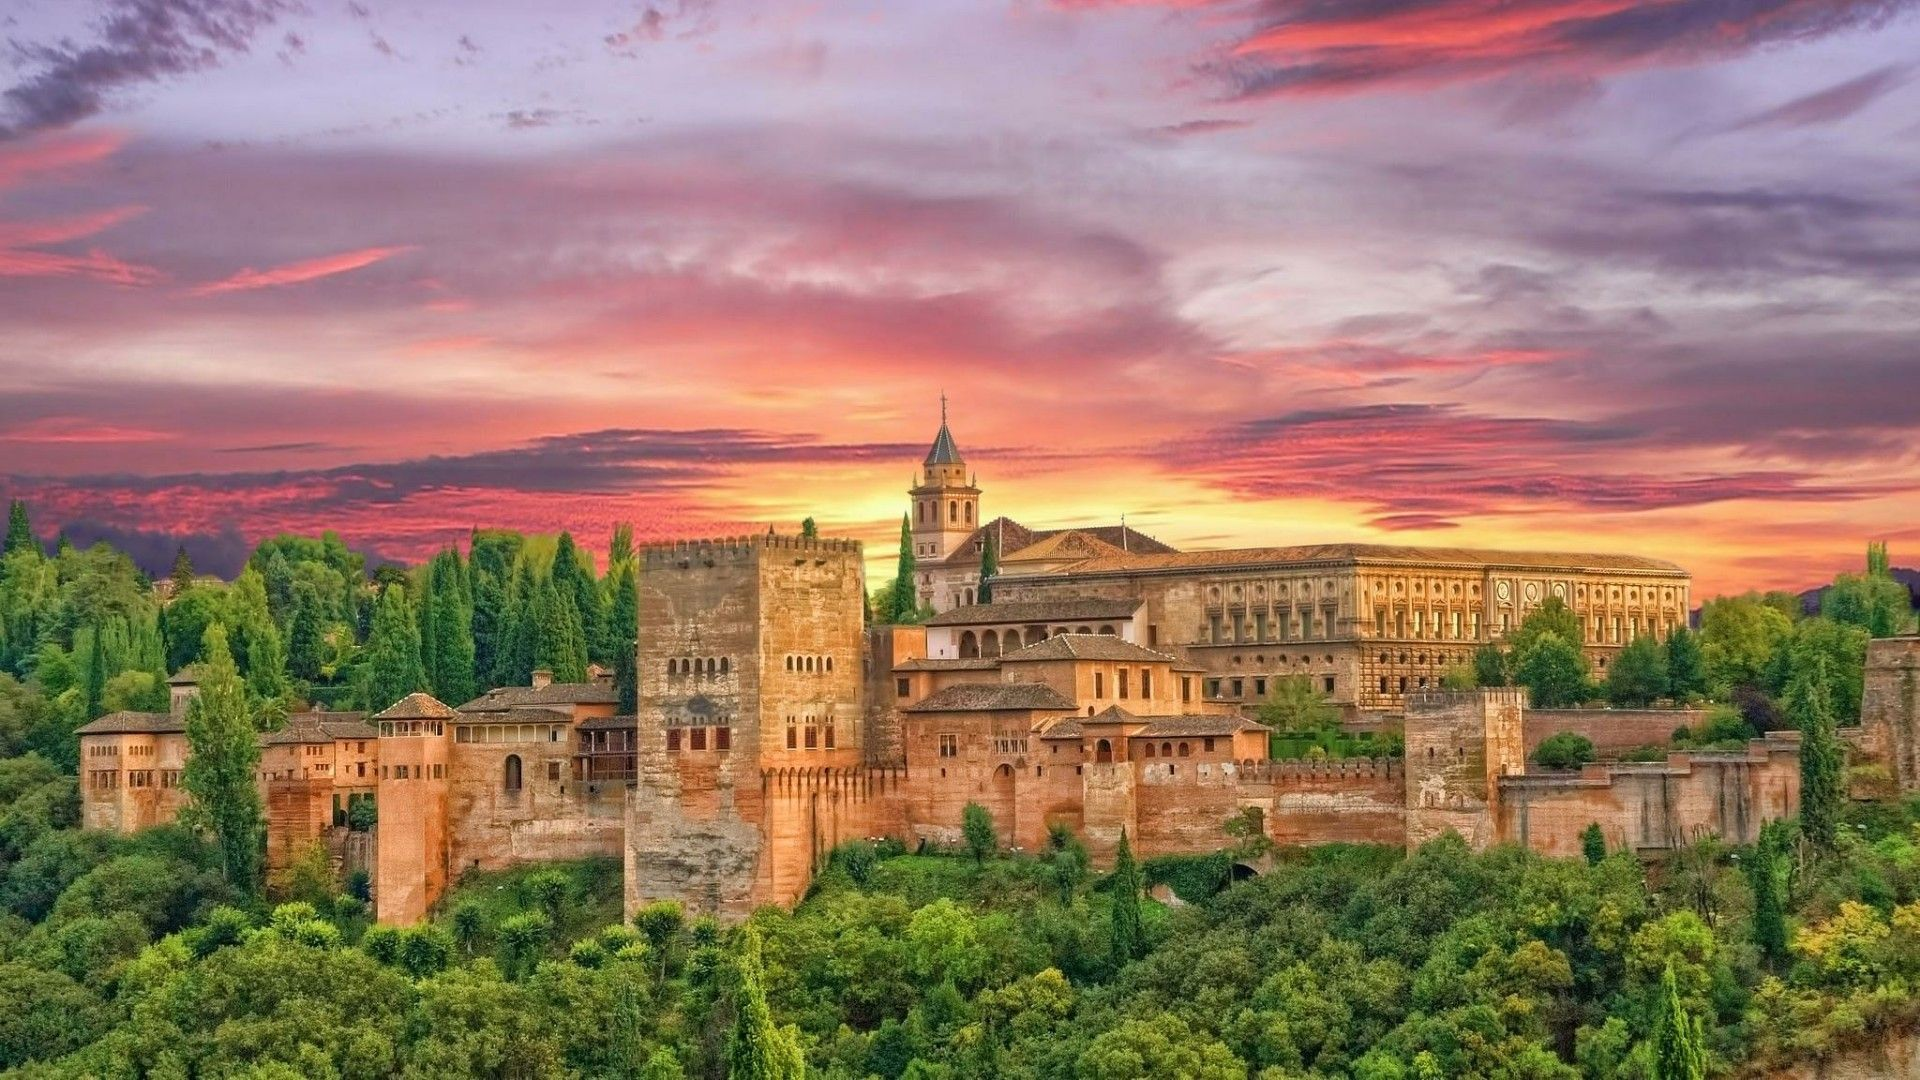
\includegraphics[width=\paperwidth,height=\paperheight,keepaspectratio]{images/granada.jpg}}
}

\usetikzlibrary{positioning}

% Inicio del documento
\begin{document}

% Portada
\maketitle
\thispagestyle{empty}

\begin{center}
    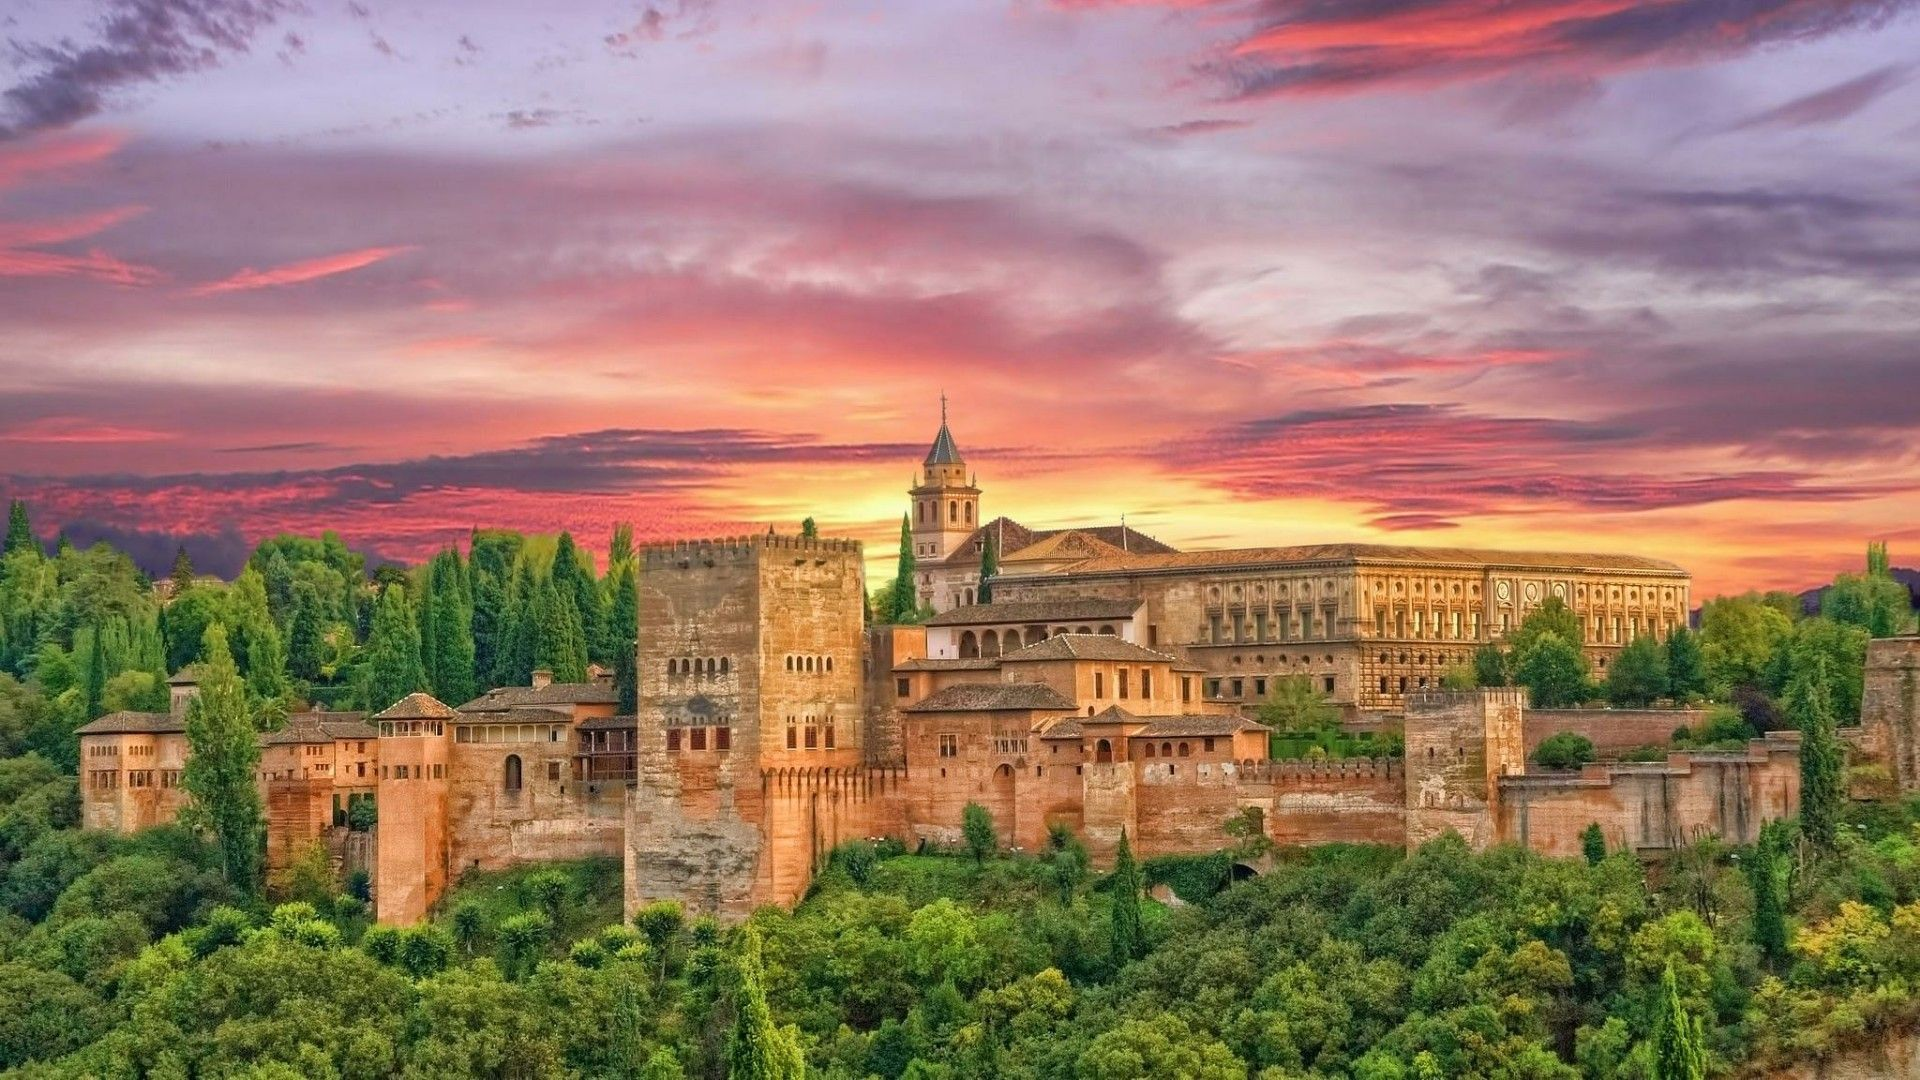
\includegraphics[width=\textwidth,height=0.4\textheight,keepaspectratio]{images/granada.jpg} \\ % Añade tu imagen de fondo
    \vfill
\end{center}

\newpage

% Índice (opcional)
\tableofcontents
\newpage

\section{Ejercicio 1}
\subsection{Enunciado}




Dada la siguiente clase en Java:

\begin{lstlisting}[style=customjava]
public class Vertebrado
{
    public ArrayList<String> partesDelAbdomen();
    public void desplazarse();
    public String comunicarse(Vertebrado vertebrado);
    protected Vertebrado obtenerCopia();
}
\end{lstlisting}

Indica con una cruz en la casilla correspondiente según si la declaración de los siguientes métodos de la clase \texttt{Mamifero}, subclase de \texttt{Vertebrado}, sobrecargan (\emph{overloading}) o redefinen (\emph{overriding}) a los de la clase \texttt{Vertebrado}.

\subsection{Solución}


\begin{table}[H]
    \centering
    \begin{tabular}{|l|c|c|}
    \hline
    \textbf{Método} & \textbf{Sobrecarga} & \textbf{Redefinición} \\ \hline
    public ArrayList<String> partesDelAbdomen() &  & X \\ \hline
    public void desplazarse(Modo m) & X &  \\ \hline
    public String comunicarse(Vertebrado vertebrado) &  & X \\ \hline
    public String comunicarse(Mamifero mamifero) & X &  \\ \hline
    public Vertebrado obtenerCopia() &  & X \\ \hline
    protected Mamiero obtenerCopia() &  & X \\ \hline
    \end{tabular}
\end{table}

\textit{Nota:Al cambiar únicamente la visibilidad o el tipo hace que sea una redefición (Últimos dos casos)}
    

\section{Ejercicio 2}
\subsection{Enunciado}




A partir de las siguientes clases:

\begin{lstlisting}[style=customjava]
public class Persona {
    protected String nombre;
    public Persona(String nom) { this.setNombre(nom); }
    protected String getNombre() { return this.nombre; }
    public String hablar() { return "bla bla bla"; }
}
\end{lstlisting}

\begin{lstlisting}[style=customjava]
public class Estudiante extends Persona {
    public String carrera;
    public int curso;
    public Estudiante(String nom, String carr, int cur) {
        super(nom);
        carrera = carr;
        curso = cur;
    }
    public void estudiar() { System.out.println("estudiando"); }
}
\end{lstlisting}

Implementa la clase \texttt{EstudianteInformatica} que hereda de \texttt{Estudiante}. Debe tener:

\begin{itemize}
    \item Una nueva variable de instancia que es una colección de \texttt{String} con los dispositivos que utiliza (por ejemplo, \texttt{PC}, \texttt{tablet}, \texttt{smartphone}).
    \item Métodos para consultar esa variable.
    \item Una redefinición del método \texttt{estudiar()} para que además de estudiar como los otros alumnos, diga que estudia con el último dispositivo de su colección.
    \item Un constructor para inicializar la clase.
\end{itemize}

Implementa este problema en Java y Ruby:

% \textbf{Implementación en Java:}

% \begin{lstlisting}[style=customjava]
% public class EstudianteInformatica extends Estudiante {
%     private ArrayList<String> dispositivos;

%     public EstudianteInformatica(String nom, String carr, int cur, ArrayList<String> dispositivos) {
%         super(nom, carr, cur);
%         this.dispositivos = dispositivos;
%     }

%     public ArrayList<String> getDispositivos() {
%         return this.dispositivos;
%     }

%     @Override
%     public void estudiar() {
%         super.estudiar();
%         if (!dispositivos.isEmpty()) {
%             System.out.println("Estudiando con " + dispositivos.get(dispositivos.size() - 1));
%         }
%     }
% }
% \end{lstlisting}

% \textbf{Implementación en Ruby:}

% \begin{lstlisting}[style=customrb]
% class Persona
%     attr_accessor :nombre

%     def initialize(nombre)
%         @nombre = nombre
%     end

%     def hablar
%         "bla bla bla"
%     end
% end

% class Estudiante < Persona
%     attr_accessor :carrera, :curso

%     def initialize(nombre, carrera, curso)
%         super(nombre)
%         @carrera = carrera
%         @curso = curso
%     end

%     def estudiar
%         puts "estudiando"
%     end
% end

% class EstudianteInformatica < Estudiante
%     attr_accessor :dispositivos

%     def initialize(nombre, carrera, curso, dispositivos)
%         super(nombre, carrera, curso)
%         @dispositivos = dispositivos
%     end

%     def estudiar
%         super
%         puts "Estudiando con #{@dispositivos.last}" unless @dispositivos.empty?
%     end
% end
% \end{lstlisting}

\subsection{Solución}

\begin{lstlisting}[style=customjava, caption={Clase Estudiante de Informática}]
    public class EstudianteInformatica extends Estudiante {
        private ArrayList<String> dispositivos;
        public EstudianteInformatica(string nombre, string curso){
            super(nombre, "Informatica", curso);
            dispositivos = new ArrayList<String>();
        }

        @Override
        public void Estudiar(){
            System.out.println("Estudiando Informatica con " + dispositivos.get(dispositivos.size() - 1));
        }
    } // Fin de la clase EstudianteInformatica
    
\end{lstlisting}

\begin{lstlisting}[style=customrb, caption={Clase Estudiante de Informática}]
    def EstudianteInformatica < Estudiante 
        def initialize (nombre, curso)
            super(nombre, "Informatica", curso)
            @dispositivos = [] # @dispositivos = Array.new
        end

        def Estudiar
            super.Estudiar
            puts "Estudiando Informatica con #{@dispositivos[-1]}"
        end
    end


\end{lstlisting}


\section{Ejercicio 3 }
\subsection{Enunciado}


\textit{Nota: En las diapositivas de la Relación hay un error, donde pone 3, no es el ejercicio 3 es la parte 2 del ejercicio 2, es decir, otra clase, el ejercicio 3 es el marcado con el número 4.}


Dada la siguiente clase abstracta en Java:

\begin{lstlisting}[style=customjava]
abstract class Transporte {
    protected String marca;

    protected String getMarca() {
        return this.marca;
    }

    protected void setMarca(String marc) {
        this.marca = marc;
    }

    public abstract String hacerRuta(String origen, String destino);
}
\end{lstlisting}

Crea dos nuevas clases, \texttt{Bicicleta} y \texttt{NaveEspacial}, que hereden de \texttt{Transporte} e implementen el método \texttt{hacerRuta} de forma diferente:

\subsection{Solución}


\begin{lstlisting}[style=customjava, caption={Clase Bicicleta}]
    public class Bicicleta extends Transporte {
        @Override
        public String hacerRuta(String origen, String destino) {
            return "Pedaleando desde " + origen + " hasta " + destino;
        }
    }

    def NaveEspacial < Transporte 
        def hacerRuta(origen, destino)
            "Volando desde #{origen} hasta #{destino} por el espacio"
        end
    end
    
\end{lstlisting}

\subsection*{Diagrama UML}

\begin{center}
\begin{tikzpicture}[node distance=2.5cm, auto]

% Main class
\node[class] (Transporte) {\textbf{Transporte}};

% Subclasses
\node[class, below left=1.5cm and 1.5cm of Transporte] (Bicicleta) {\textbf{Bicicleta}};
\node[class, below right=1.5cm and 1.5cm of Transporte] (NaveEspacial) {\textbf{NaveEspacial}};

% Arrows
\draw[arrow] (Bicicleta.north) -- (Transporte.south west);
\draw[arrow] (NaveEspacial.north) -- (Transporte.south east);

\end{tikzpicture}
\end{center}

\newpage
\section{Ejercicio 4} 
\subsection{Enunciado}
Hacer el ejercicio anterior, pero en Ruby.
\subsection{Solución}


\begin{lstlisting}[style=customrb, caption={Clase Bicicleta}]
    def Bicicleta < Transporte 
        def hacerRuta(origen, destino)
            "Pedaleando desde #{origen} hasta #{destino}"
        end
    end

    def NaveEspacial < Transporte 
        def hacerRuta(origen, destino)
            "Volando desde #{origen} hasta #{destino} por el espacio"
        end
    end
\end{lstlisting}

\subsection{Enunciado}

Implementa en Java una clase paramétrica a partir de la cual se puedan definir clases de grupos de personas con un líder, como por ejemplo grupos de música con un cantante, o empresas con un jefe. Implementa también alguna de esas clases a partir de la clase paramétrica definida.

\subsection{Solución}

A continuación, se implementa una clase paramétrica en Java para definir grupos de personas con un líder. Posteriormente, se muestra un ejemplo de uso creando un grupo de música con un cantante.

\begin{lstlisting}[style=customjava]
// Clase paramétrica genérica
public class Grupo<T> {
    private T lider;
    private List<T> miembros;

    public Grupo(T lider) {
        this.lider = lider;
        this.miembros = new ArrayList<>();
    }

    public T getLider() {
        return lider;
    }

    public void setLider(T lider) {
        this.lider = lider;
    }

    public void agregarMiembro(T miembro) {
        this.miembros.add(miembro);
    }

    public List<T> getMiembros() {
        return miembros;
    }

    @Override
    public String toString() {
        return "Líder: " + lider + ", Miembros: " + miembros;
    }
}

// Ejemplo de uso con un grupo de música
public class Musico {
    private String nombre;

    public Musico(String nombre) {
        this.nombre = nombre;
    }

    @Override
    public String toString() {
        return nombre;
    }
}

public class Main {
    public static void main(String[] args) {
        Musico cantante = new Musico("Freddie Mercury");
        Grupo<Musico> banda = new Grupo<>(cantante);
        
        banda.agregarMiembro(new Musico("Brian May"));
        banda.agregarMiembro(new Musico("Roger Taylor"));
        banda.agregarMiembro(new Musico("John Deacon"));

        System.out.println(banda);
    }
}
\end{lstlisting}

Si queremos implementar esta misma solución en Ruby, sería como sigue:

\begin{lstlisting}[style=customrb]
# Clase paramétrica genérica
class Grupo
  attr_accessor :lider, :miembros

  def initialize(lider)
    @lider = lider
    @miembros = []
  end

  def agregar_miembro(miembro)
    @miembros << miembro
  end

  def to_s
    "Líder: #{@lider}, Miembros: #{@miembros.join(', ')}"
  end
end

# Ejemplo de uso con un grupo de música
class Musico
  attr_accessor :nombre

  def initialize(nombre)
    @nombre = nombre
  end

  def to_s
    @nombre
  end
end

# Crear grupo de música
cantante = Musico.new("Freddie Mercury")
banda = Grupo.new(cantante)

banda.agregar_miembro(Musico.new("Brian May"))
banda.agregar_miembro(Musico.new("Roger Taylor"))
banda.agregar_miembro(Musico.new("John Deacon"))

puts banda
\end{lstlisting}

\section{Ejercicio 6}
\subsection{Enunciado}
Partiendo del siguiente diagrama de clases, modifícalo añadiendo una interfaz Prestable
implementada por la clase ElementoPrestable y sus subclases. Añade a este diagrama de
clases los atributos y operaciones de las distintas clases y de la interfaz Prestable.

% \begin{figure}[H]
%     \centering
%     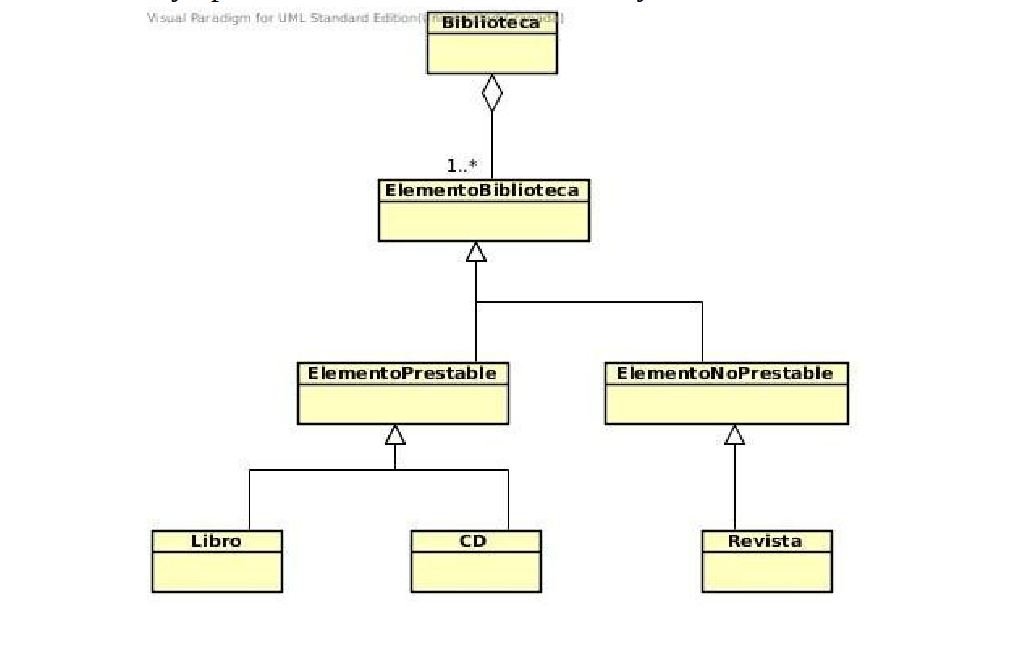
\includegraphics[width=0.9\textwidth]{images/ej7.png}
%     \caption{Diagrama de clases}
%     \label{fig:ejercicio6}
% \end{figure}

\begin{center}
    \begin{tikzpicture}[node distance=0.8cm, auto, scale=0.75, transform shape]
    
    % Main class
    \node[class] (Biblioteca) {\textbf{Biblioteca}};
    
    % Subclass
    \node[class, below=0.4cm of Biblioteca] (ElementoBiblioteca) {\textbf{ElementoBiblioteca}};
    \node[right=0.00001cm of ElementoBiblioteca] {1...*};
    
    % Subclasses of ElementoBiblioteca
    \node[class, below left=0.4cm and 0.4cm of ElementoBiblioteca] (ElementoPrestable) {\textbf{ElementoPrestable}};
    \node[class, below right=0.4cm and 0.4cm of ElementoBiblioteca] (ElementoNoPrestable) {\textbf{ElementoNoPrestable}};
    
    % Subclasses of ElementoPrestable
    \node[class, below left=0.4cm and 0.4cm of ElementoPrestable] (Libro) {\textbf{Libro}};
    \node[class, below right=0.4cm and 0.4cm of ElementoPrestable] (CD) {\textbf{CD}};
    
    % Subclass of ElementoNoPrestable
    \node[class, below=0.4cm of ElementoNoPrestable] (Revista) {\textbf{Revista}};
    
    % Arrows
    \draw[arrow] (ElementoBiblioteca.north) -- (Biblioteca.south);
    \draw[arrow] (ElementoPrestable.north) -- (ElementoBiblioteca.south west);
    \draw[arrow] (ElementoNoPrestable.north) -- (ElementoBiblioteca.south east);
    \draw[arrow] (Libro.north) -- (ElementoPrestable.south west);
    \draw[arrow] (CD.north) -- (ElementoPrestable.south east);
    \draw[arrow] (Revista.north) -- (ElementoNoPrestable.south);
    
    \end{tikzpicture}
\end{center}


\subsection{Solución}

\begin{center}
    \begin{tikzpicture}[node distance=0.8cm, auto, scale=0.75, transform shape]

    % Define the style for the classes
    \tikzstyle{class} = [rectangle, draw, text width=4cm, text centered, rounded corners, minimum height=2em]
    \tikzstyle{diamondline} = [thick, -{Diamond[open, scale=1.5]}]
    
    %Main class
    \node[class] (Biblioteca) {\textbf{Biblioteca} \\ \textit{+elementos: ElementoBiblioteca[] }};    
        

    % Subclass
    \node[class, below=0.6cm of Biblioteca] (ElementoBiblioteca) {\textbf{ElementoBiblioteca} +titulo: String \\ +autor: String \\ +prestado: boolean \\ +fechaPrestamo: Date \\ +fechaDevolucion: Date \\ +prestar() \\ +devolver() \\ +estaPrestado() \\ +tiempoPrestamo() \\ +toString()};
    \node[above right=0.00001cm of ElementoBiblioteca] {1...*};
    
    % Subclasses of ElementoBiblioteca
    \node[class, below left=0.4cm and 0.4cm of ElementoBiblioteca] (interfacePrestable) {\textbf{Interfaz Prestable} \\ +prestar() \\ +devolver() \\ +estaPrestado() \\ +tiempoPrestamo() \\ +toString()};
    \node[class, below right=0.4cm and 0.4cm of ElementoBiblioteca] (ElementoNoPrestable) {\textbf{ElementoNoPrestable} +tipo: String \\ +toString()};

    % Subclasses of interfacePrestable
    \node[class, below left=0.4cm and 0.4cm of interfacePrestable] (ElementoPrestable) {\textbf{ElementoPrestable} \\ +prestar() \\ +devolver() \\ +estaPrestado() \\ +tiempoPrestamo() \\ +toString()};
    
    % Subclasses of ElementoPrestable
    \node[class, below left=0.4cm and 0.4cm of ElementoPrestable] (Libro) {\textbf{Libro} +numPaginas: int \\ +toString()};
    \node[class, below right=0.4cm and 0.4cm of ElementoPrestable] (CD) {\textbf{CD} +duracion: int \\ +toString()};
    
    % Subclass of ElementoNoPrestable
    \node[class, below=0.4cm of ElementoNoPrestable] (Revista) {\textbf{Revista} +periodicidad: String \\ +toString()};
    
    % Arrows
    \draw[diamondline] (ElementoBiblioteca.north) -- (Biblioteca.south);
    \draw[arrow] (interfacePrestable.north) -- (ElementoBiblioteca.south west);
    \draw[arrow] (ElementoPrestable.north) -- (interfacePrestable.south west);
    \draw[arrow] (ElementoNoPrestable.north) -- (ElementoBiblioteca.south east);
    \draw[arrow] (Libro.north) -- (ElementoPrestable.south west);
    \draw[arrow] (CD.north) -- (ElementoPrestable.south east);
    \draw[arrow] (Revista.north) -- (ElementoNoPrestable.south);
    
    \end{tikzpicture}
\end{center}



\end{document}